\documentclass[a5paper,12pt]{article}
\usepackage{../../style}


\newcommand{\montitre}{Algo }


\begin{document}

\fiche{Introduction}
\titre{Biblio :} Cormen, Intro à l'algorithmique \\

\titre{Prérequis :}
\begin{itemize}
	\item Complexité asymptotique en pire cas
	\item Notation $O(), \theta(), \Omega()$
	\item \begin{itemize}
		\item $\theta(\ln n)$ : algo (poly)logarithmique
		\item $\theta(n)$ : algo linéaire (min ou max d'un tableau)
		\item $\theta(n\ln n)$ : algo quasi linéaire (tri par tas)
		\item $\theta(n^2)$ : algo quadratique (tri par insertion, tri bulle)
		\item $\theta(n^3)$ : algo cubique (calcul de tous les plus courts chemins dans un graphe)
		\item $\theta(2^n)$ : voyageur de commerce (pas sur, peut être en $\theta(n^k)$)
		\item $\theta(n!)$ : Bogo-sort
	\end{itemize}
\end{itemize}

\titre{Ce qu'on va faire :}
\begin{itemize}
	\item Analyse des algos récursifs
	\item Analyse amortie
\end{itemize}


\fiche{Connexité}
\titre{Chemin :} Un chemin dans un graphe $G=(S,A)$ est une séquence de sommets $C = [ c_1,\ldots,c_n ]$ telle que $(c_i,c_{i+1}) \in A \forall i \in \{ 1 .. n-1 \}$ \\
 
\titre{Longueur :} La longueur de $C$ est $n-1$ \\

\titre{Chemin simple :} $i\neq j \impl c_i \neq c_j$ \\

\titre{Cycle :} Un cycle est un chemin "simple" mais avec $c_1 = c_n$, sauf les chemins du type $[u,v,u]$ des graphes non orientés. \\

\titre{Critère d'isomorphie :} Deux graphes isomorphes ont le même nombre de cycles de chaque longueur. Ce critère est nécessaire mais non suffisant. (fig6)\\

\titre{Condition nécessaire :} \\
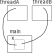
\includegraphics[width=100px]{Images/fig4.pdf} \hspace{1cm} 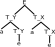
\includegraphics[width=100px]{Images/fig5.pdf} \\

\titre{Condition non suffisante :} \\

\includegraphics[width=100px]{Images/fig6.pdf} \\

\titre{Composante connexe :} Soit $G=(S,A)$ un graphe non orienté. Une commposante connexe de $G$ est un sous ensemble maximal de sommets $S'$ tel que pour toute paire de sommets $(u,v)$ de $S'$, il existe un chemin de $u$ à $v$. \\

\titre{Connexité :} Un graphe est dit connexe s'il ne contient qu'une seule composante connexe. \\

\titre{Composante fortement connexe :} Soit $G=(S,A)$ un graphe orienté. Une commposante fortement connexe de $G$ est un sous ensemble maximal de sommets $S'$ tel que pour toute paire de sommets $(u,v)$ de $S'$, il existe un chemin de $u$ à $v$. \\

\titre{Graphe fortement connexe :} Ses sommets forment une composante fortement connexe. \\



\fiche{Arbres}
\input{Includes/03_Arbres.tex}

\fiche{Parcours de graphes}
\input{Includes/04_ParcoursGraphes.tex}

\fiche{TD 1}
\titre{Question 1}\\
\\
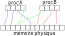
\includegraphics{Images/fig19.pdf}
\\
\newpage
\titre{Question 2}\\
\\
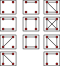
\includegraphics[width=200px]{Images/fig20.pdf}
\\
\\
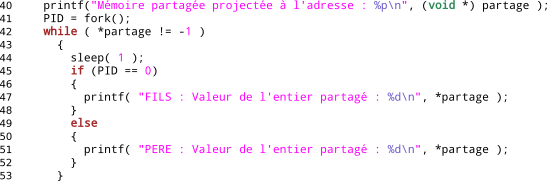
\includegraphics[width=300px]{Images/fig21.pdf}
\\
\titre{Question 3}
\begin{enumerate}
	\item $K_n$ possède $\frac{n(n-1)}{2}$ arêtes.
	\item $\bar{K_n}$ possède 0 arête
	\item $O(n^2)$
\end{enumerate}

\titre{Question 4} Il y a deux sous graphes isomorphes à $K_3$ et aucun isomorphe à $\bar{K_3}$
\newpage
\titre{Question 5} \\
\\

\includegraphics[width=100px]{Images/fig23.pdf}
\\
\titre{Question 6} 
\begin{enumerate}
	\item .\\ 
\includegraphics{Images/fig24.pdf}
	\item $O(n^2)$
	\item .\\
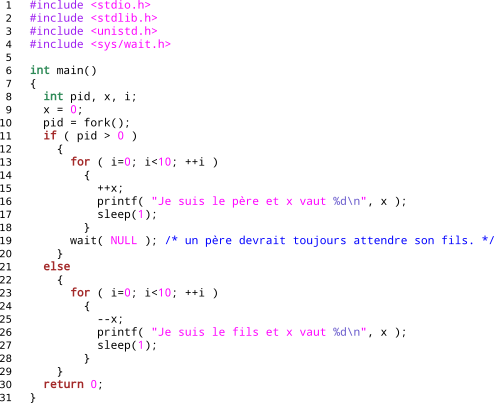
\includegraphics{Images/fig25.pdf}
	\item $O(n^2)$
	\item Faire mieux ???
\end{enumerate}

\titre{Question 7} Il faut commencer par enlever une allumette \\
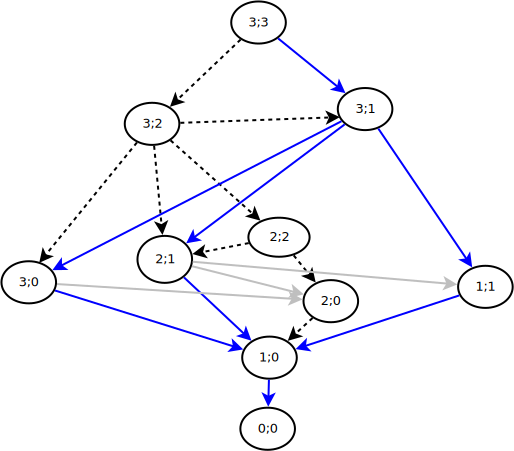
\includegraphics[width=250px]{Images/fig26.pdf} \\

\titre{Question 8} P = passeur, C = choux, B = chèvre (bêêê), L = loup \\
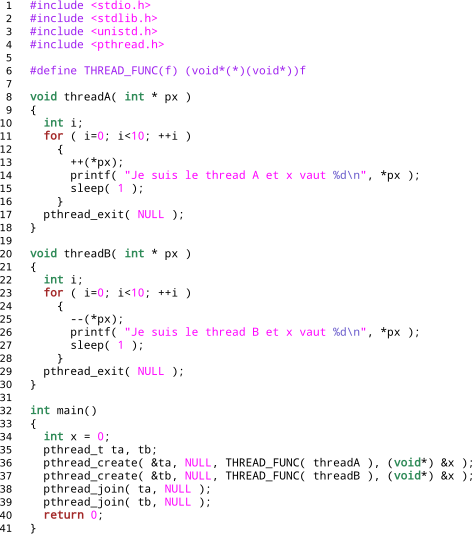
\includegraphics[width=250px]{Images/fig27.pdf} \\

\titre{Question 9} \\
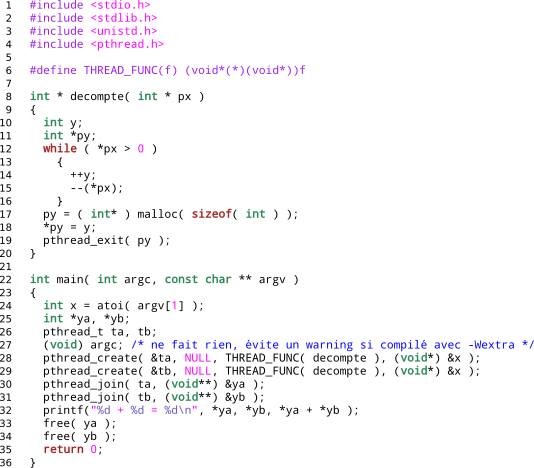
\includegraphics[width=300px]{Images/fig28.pdf} \\


\fiche{TD 2}
\input{Includes/06_TD2.tex}

\fiche{Chemins de longueur minimale}
\titre{Calcul des CLM : Chemins de Longueur Minimale}
\begin{enumerate}
	\item D'un sommet à un autre (on fait le 2 et on extrait le bon chemin)
	\item D'un sommet à tous les autres (Dijkstra)
	\item De tous les sommets à un autre (On inverse les arêtes du graphe et on fait 2)
	\item De tous les sommets vers tous les sommets (Floyd-Warshall)
\end{enumerate}

\titre{Définition :} Soit $G=(S,A)$ un graphe et $p$ sa fonction de pondération. Un \titre{Chemin de Longueur Minimale} du sommet $u$ au sommet $v$ est un chemin de $[s_0,\ldots,s_k]$ avec $s_0=u$, $s_k=v$ et $\sum p(s_i,s_{i+1})$ minimal.\\

\titre{Arbre de CLM :} Un arbre couvrant enraciné en un sommet $s$ tel que l'unique chemin de $s$ à un sommet $u$ de cet arbre est un CLM du graphe de départ. \\

\titre{Remarques :} 
\begin{itemize} 
	\item L'arbre de CLM existe.
	\item Soit $[s_0,\ldots,s_k]$ un CLM de $s_0$ à $s_k$. Alors pour tout $i\in\{1,\ldots,k-1\}$ on a $[s_0,\ldots s_i]$ est un CLM de $s_0$ à $s_i$
\end{itemize}

\titre{Algorithme de Dijkstra :} Meme principe que l'algo de Prim à la différence que cle[u] est la longueur du plus court chemin connu du sommet de départ au sommet u.\\

\titre{Algorithme de Floyd-Warshall :} L'idée est de construire dynamiquement une suite de matrices $M_0,\ldots,M_n$ telles que $m_{k_{i,j}}$ est le cout du plus court chemine de $i$ à $j$ en utilisant comme sommets intermédiaires les sommets $1,2,\ldots ,k$


\fiche{Problèmes de maximisation}
\input{Includes/08_Maximisation.tex}

\end{document}
